\documentclass[acmsmall,screen,nonacm]{acmart}

% Ρυθμίσεις Γλώσσας και Γραμματοσειρών
\usepackage[greek,english]{babel}
\usepackage{alphabeta} 
\usepackage{amsmath}
\usepackage{algorithm}
\usepackage{algpseudocode}

\sloppy % Βοηθάει στην στοίχιση του κειμένου

% Τίτλος και Στοιχεία
\title{Dynamic Scenes}
\subtitle{3D Υπολογιστική Γεωμετρία \& Όραση }

\author{Δημήτριος Φιλόπουλος}
\affiliation{
	\institution{Τμήμα ΗΜ\&ΤΥ, Πανεπιστήμιο Πατρών}
	\country{Ελλάδα}
}

\renewcommand{\shortauthors}{Δ.Φ}

\begin{document}
	
	\maketitle
	
	\section{Εισαγωγή}
	
	\subsection{Σκοπός της Εργασίας}
	Σκοπός της παρούσας εργασίας είναι η φόρτωση και η ανάλυση 3D νεφών Σημείων για την ανίχνευση χωρικών και γεωμετρικών αλλαγών μεταξύ διαφορετικών χρονικών εποχών. Η διαδικασία αυτή περιλαμβάνει το φιλτράρισμα του εδάφους, την ευθυγράμμιση των δεδομένων, τη χωρική διαμέριση με Quadtree και Octree, καθώς και τη κατηγοριοποίηση των διαφορετικών αντικειμένων της σκηνής.
	
	\subsection{Αρχιτεκτονική και Εργαλεία Ανάπτυξης}
	Για την υλοποίηση της εργασίας χρησιμοποιήθηκε η γλώσσα προγραμματισμού Python 3.12 με την χρήση της βιβλιοθήκης \texttt{vvrpywork}. Επιπλέον, χρησιμοποιήθηκαν οι εξής βιβλιοθήκες:
	\begin{itemize}
		\item \textbf{NumPy:} για τον γρήγορο υπολογισμό των μαθηματικών.
		\item \textbf{Laspy:} για την ανάγνωση των νεφών σημείων από αρχεία μορφής \texttt{.las} και \texttt{.laz}.
		\item \textbf{PyQt5:} για τη δημιουργία της γραφικής διεπαφής και τη διαχείριση ασύγχρονων νημάτων στο παρασκήνιο για την επεξεργασία των δεδομένων.
	\end{itemize}


	\section{Φόρτωση, Φιλτράρισμα και Αφαίρεση Εδάφους}
	Το πρώτο στάδιο της επεξεργασίας αφορά τη φόρτωση και την κατάλληλη προετοιμασία των σημείων.
	
	\subsection{Ανάγνωση Δεδομένων}
	Στην εργασία αυτή διαχειριζόμαστε δύο διαφορετικά είδη δεδομένων: δεδομένα από σταθερό LiDAR (αρχεία μορφής \texttt{.laz}) και δεδομένα από LiDAR τοποθετημένο σε κινούμενο αυτοκίνητο (ακολουθία αρχείων \texttt{.pcd}).
	
	Τα δεδομένα \texttt{.laz} φορτώνονται απευθείας από το αρχικό αρχείο χρησιμοποιώντας τη βιβλιοθήκη Laspy. Αντίθετα, για τα δεδομένα \texttt{.pcd}, η ανάγνωση γίνεται με τη βοήθεια ενός αρχείου (\texttt{calibration.csv}), το οποίο περιέχει τη συσχέτιση κάθε αρχείου σημείων με τον αντίστοιχο πίνακα γεωμετρικού μετασχηματισμού του.
	
	\begin{figure}[h!]
		\centering
		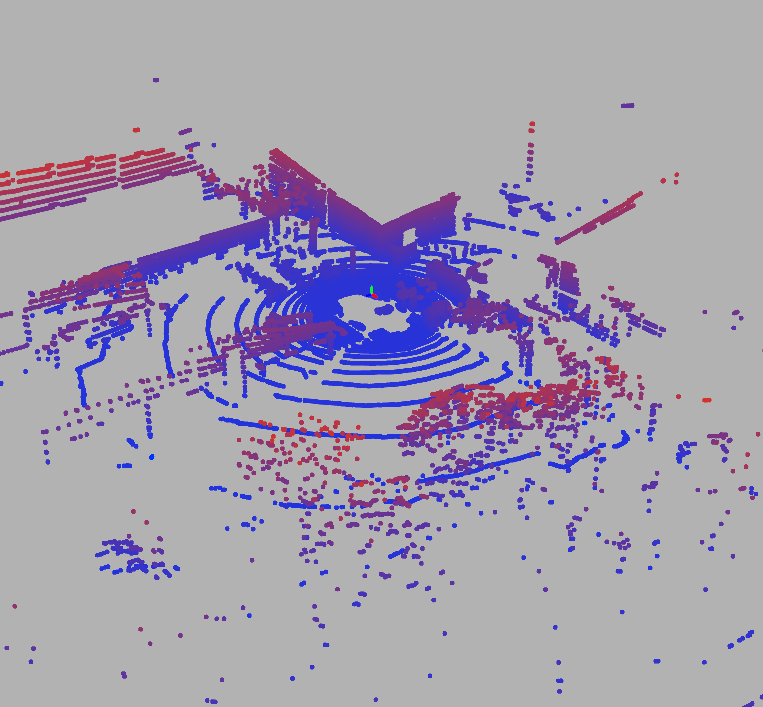
\includegraphics[width=0.8\textwidth]{images/raw_pointcloud.png}
		\caption{Αρχικό νέφος σημείων LiDAR πριν από την επεξεργασία και την αφαίρεση του εδάφους.}
		\label{fig:raw_pointcloud}
	\end{figure}
	
	\subsection{Αφαίρεση Εδάφους με Φίλτρο Τοπικού Ελαχίστου}
	Κατά τη φάση της προετοιμασίας, αφαιρούμε το έδαφος για να διευκολύνουμε την ανίχνευση αλλαγών. Επιπλέον, πραγματοποιούμε downsampling στα μεγάλα σε όγκο δεδομένα LiDAR, προκειμένου να βελτιστοποιήσουμε την ταχύτητα επεξεργασίας και το rendering της τρισδιάστατης σκηνής.
	
	Η αφαίρεση του εδάφους γίνεται με τον εξής τρόπο:
	\begin{itemize}
		\item Υπολογίζουμε αρχικά μια σταθερά με βάση το 2ο εκατοστημόριο της κατανομής του ύψους όλων των σημείων (δηλαδή το ύψος όπου το 98\% των σημείων είναι μεγαλύτερο).
		\item Χωρίζουμε την οριζόντια επιφάνεια σε ένα δισδιάστατο πλέγμα με κελιά σταθερού μεγέθους.
		\item Για κάθε κελί, βρίσκουμε το τοπικό ελάχιστο ύψος (5ο εκατοστημόριο του ύψους των σημείων του κελιού).
		\item Εάν το τοπικό ελάχιστο ενός κελιού είναι μεγαλύτερο από το παγκόσμιο, ορίζουμε ως ύψος εδάφους του κελιού το παγκόσμιο υψόμετρο.
		\item Διατηρούμε μόνο τα σημεία που έχουν ύψος μεγαλύτερο από το τελικό ύψος εδάφους του κελιού τους συν ένα μικρή τιμή.
	\end{itemize}
	Με αυτόν τον τρόπο απομονώνουμε επιτυχώς τις υπεργείες δομές ενδιαφέροντος και μειώνουμε τον υπολογιστικό φόρτο των επόμενων σταδίων.
	
	\begin{figure}[h!]
		\centering
		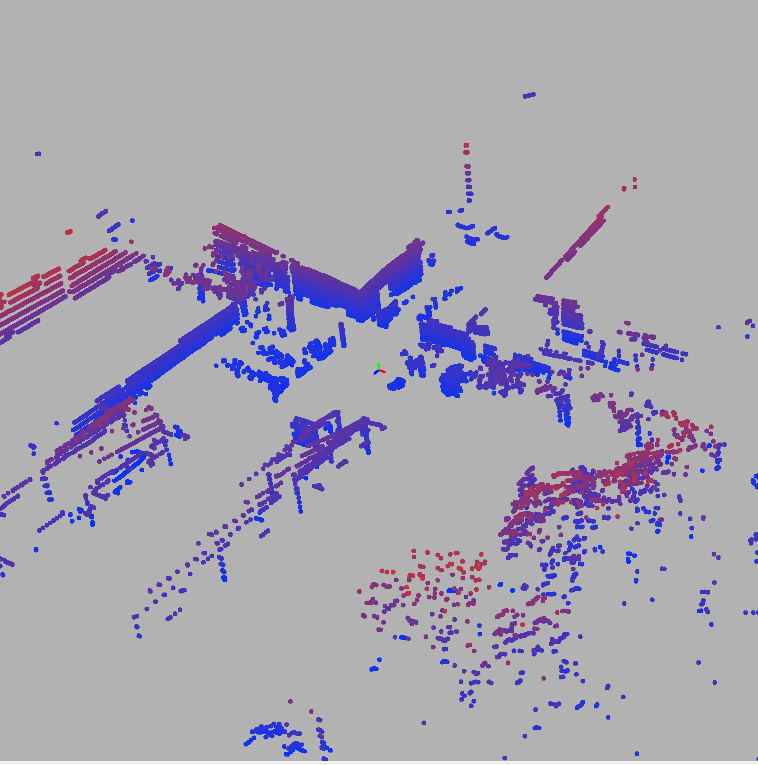
\includegraphics[width=0.8\textwidth]{images/clean_pointcloud.png}
		\caption{Εφαρμογή φίλτρου τοπικού ελαχίστου για αφαίρεση εδάφους.}
		\label{fig:clean_pointcloud}
	\end{figure}

	\section{Ευθυγράμμιση και Καταχώριση Νεφών Σημείων}
	Η διαδικασία αυτή εφαρμόζεται αποκλειστικά στα δεδομένα σταθερού LiDAR (αρχεία \texttt{.laz}). Αντίθετα, η ακολουθία των αρχείων \texttt{.pcd} ευθυγραμμίζεται απευθείας κατά τη φόρτωση χρησιμοποιώντας τους έτοιμους πίνακες μετασχηματισμού από το αρχείο .csv.
	
	\subsection{Αρχική Προσέγγιση με PCA}
	 Για την αρχική ευθυγράμμιση των δεδομένων χρησιμοποιούμε τη μέθοδο PCA. Επειδή το ύψος είναι ήδη ευθυγραμμισμένο, κάνουμε PCA μόνο στο οριζόντιο επίπεδο κρατώντας το ύψος σταθερό, για να αποφύγουμε να γυρίσει το έδαφος ανάποδα. Υπολογίζουμε τα κύρια ιδιοδιανύσματα για να βρούμε την περιστροφή και στη συνέχεια μετατοπίζουμε και περιστρέφουμε τα σημεία ώστε να έρθουν χονδρικά κοντά.
	
	\subsection{Λεπτομερής Ευθυγράμμιση με ICP}
	Για την τελική και ακριβή ευθυγράμμιση εφαρμόζουμε τον αλγόριθμο ICP:
	\begin{itemize}
		\item Για κάθε σημείο του πρώτου νέφους, βρίσκουμε το πιο κοντινό του σημείο στο δεύτερο νέφος.
		\item Υπολογίζουμε την περιστροφή και τη μετατόπιση που ελαχιστοποιεί την απόσταση μεταξύ τους χρησιμοποιώντας SVD.
		\item Εφαρμόζουμε αυτόν τον μετασχηματισμό στα σημεία του πρώτου νέφους.
		\item Επαναλαμβάνουμε τη διαδικασία μέχρι η αλλαγή στο σφάλμα (MSE) να γίνει πολύ μικρή ή να φτάσουμε έναν συγκεκριμένο αριθμό επαναλήψεων.
	\end{itemize}
	
	\begin{figure}[h!]
		\centering
		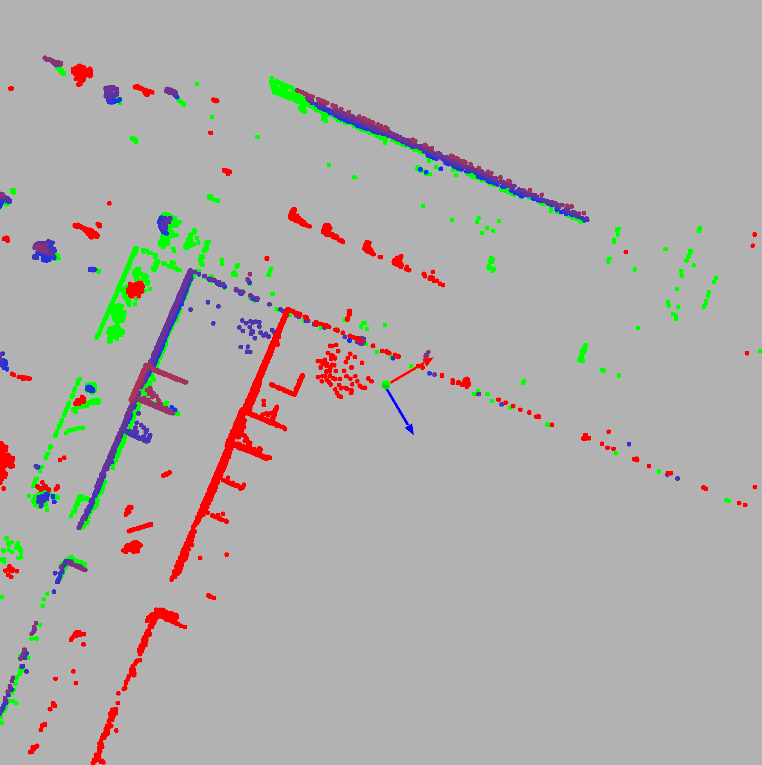
\includegraphics[width=0.8\textwidth]{images/icp.png}
		\caption{Οπτικοποίηση ευθυγράμμισης των δύο εποχών LiDAR (PCA και ICP).}
		\label{fig:alignment}
	\end{figure}
	
	\section{Ανίχνευση Μεταβολών και Διαφορών}
	
	\subsection{Διαφοροποίηση Σημείων}
	Για να βρούμε ποιες αλλαγές έγιναν στη σκηνή, συγκρίνουμε δύο διαδοχικά καρέ υπολογίζοντας τις αποστάσεις μεταξύ τους. Για την ταχύτατη εύρεση του πλησιέστερου σημείου χρησιμοποιούμε ένα \texttt{KDTree}:
	\begin{itemize}
		\item \textbf{Νέα σημεία:} Για κάθε σημείο του τρέχοντος καρέ, βρίσκουμε το πλησιέστερο σημείο του στο προηγούμενο καρέ. Αν η απόσταση είναι μεγαλύτερη από ένα όριο, το σημείο θεωρείται νέο.
		\item \textbf{Στατικά σημεία:} Αν η απόσταση είναι μικρότερη από το όριο, το σημείο θεωρείται στατικό (υπήρχε και στα 2 νέφη).
		\item \textbf{Σημεία που αφαιρέθηκαν:} Για κάθε σημείο του προηγούμενου καρέ, βρίσκουμε το πλησιέστερο σημείο του στο τρέχον καρέ. Αν η απόσταση είναι μεγαλύτερη από το όριο, το σημείο θεωρείται ότι αφαιρέθηκε (η ίδια διαδικασία ανάποδα).
	\end{itemize}
	
	\subsection{Ανίχνευση Γεωμετρικών Αλλοιώσεων και Παραμορφώσεων}
	Για να εντοπίσουμε αλλαγές στη γεωμετρία και το σχήμα των αντικειμένων, κατασκευάζουμε πρώτα ένα δέντρο (Quadtree ή Octree) για κάθε καρέ. Στη συνέχεια, συγκρίνουμε αναδρομικά τα δέντρα ξεκινώντας από τις ρίζες τους:
	\begin{itemize}
		\item \textbf{Σύγκριση Φύλλων (Leaf Nodes):} Αν φτάσουμε σε φύλλα και στα δύο δέντρα που περιέχουν σημεία, ελέγχουμε αν το σχήμα τους έχει αλλάξει χρησιμοποιώντας δύο κριτήρια:
		\begin{itemize}
			\item \textbf{PCA:} Συγκρίνουμε τις ιδιοτιμές των σημείων. Αν η διαφορά τους είναι μεγάλη, το σχήμα θεωρείται αλλοιωμένο (π.χ. αν μια επίπεδη επιφάνεια έγινε σφαιρική).
			\item \textbf{Απόσταση Hausdorff:} Υπολογίζουμε τη μέγιστη απόσταση των σημείων των δύο φύλλων. Συγκεκριμένα, βρίσκει για κάθε σημείο του ενός φύλλου την απόσταση από το πλησιέστερο σημείο του άλλου και κρατάει τη μέγιστη. Αν αυτή η μέγιστη απόσταση ξεπερνά ένα όριο, σημαίνει ότι υπάρχει κάποιο σημείο που έχει μετατοπιστεί ή παραμορφωθεί σημαντικά.
		\end{itemize}
		Αν τουλάχιστον ένα από τα δύο κριτήρια της σύγκρισης φύλλων ισχύει, τότε το φύλλο χαρακτηρίζεται ως τροποποιημένο (changed).
		\item \textbf{Προσθήκη ή Αφαίρεση:} Αν το ένα αντίστοιχο κουτί έχει σημεία και το άλλο είναι άδειο (ή το ένα είναι φύλλο και το άλλο έχει χωριστεί σε παιδιά), τότε καταγράφεται απευθείας προσθήκη ή αφαίρεση
		\item \textbf{Αναδρομή:} Αν κανένα από τα Nodes δεν είναι φύλλο, καλούμε την ίδια διαδικασία αναδρομικά για τα παιδιά τους.
	\end{itemize}
	


	\section{Ιεραρχική Χωρική Διαμέριση}
	
	\subsection{Δυαδικό Δέντρο Αναζήτησης KD-Tree}
	Το KD-Tree είναι ένα δυαδικό δέντρο διαμέρισης χώρου που χρησιμοποιείται για την ταχύτατη εύρεση πλησιέστερων γειτόνων:
	\begin{itemize}
		\item Σε κάθε επίπεδο, το δέντρο χωρίζει τα σημεία σε δύο ίσα μέρη χρησιμοποιώντας τη διάμεσο κατά μήκος ενός άξονα (X, Y ή Z).
		\item Μας επιτρέπει να κάνουμε αναζήτηση πλησιέστερου γείτονα σε χρόνο $O(\log N)$.
		\item Στην εργασία χρησιμοποιείται για την εύρεση αντιστοιχιών στον ICP, στην ανίχνευση αλλαγών, καθώς και για την απόδοση των τελικών κατηγοριών στα σημεία μετά το clustering.
	\end{itemize}
	
	\subsection{Quadtree για Περιοχές Αλλαγών}
	Το Quadtree είναι μια δομή ιεραρχικής διαμέρισης του δισδιάστατου οριζόντιου χώρου:
	\begin{itemize}
		\item Χωρίζει το επίπεδο X-Y σε 4 ίσα τεταρτημόρια.
		\item Η διαίρεση γίνεται αναδρομικά μέχρι κάθε φύλλο να περιέχει το πολύ 50 σημεία ή να φτάσει σε μέγιστο βάθος 6 επιπέδων.
		\item Χρησιμοποιείται για τον εντοπισμό περιοχών αλλαγών στο 2D επίπεδο, ομαδοποιώντας τα σημεία που προστέθηκαν ή αφαιρέθηκαν.
		\item Επειδή η αναπαράσταση γίνεται σε δύο διαστάσεις, τα bounding boxes του Quadtree είναι πολύ πιο «καθαρά» και εύκολα στο μάτι κατά την απεικόνιση του Point Cloud.
	\end{itemize}
	
	\subsection{Octree για Περιοχές Αλλαγών}
	Το Octree επεκτείνει τη λογική του Quadtree στις τρεις διαστάσεις:
	\begin{itemize}
		\item Χωρίζει τον τρισδιάστατο χώρο X-Y-Z σε 8 ίσα οκταμόρια.
		\item Η διαίρεση σταματά αναδρομικά αν ένα φύλλο περιέχει το πολύ 50 σημεία ή αν φτάσουμε σε βάθος 5 επιπέδων.
		\item Χρησιμοποιείται για τη σύγκριση των δύο εποχών σε τρισδιάστατο επίπεδο, επιτρέποντας τον εντοπισμό αλλαγών καθ' ύψος (π.χ. προσθήκη ορόφου σε ένα κτίριο).
		\item Παρόλα αυτά, η οπτικοποίηση του Octree είναι αρκετά δύσκολη στην πράξη, καθώς η προβολή πολλών τρισδιάστατων κουτιών που επικαλύπτονται δημιουργεί οπτικό θόρυβο στη σκηνή.
	\end{itemize}
	
	\begin{figure}[h!]
		\centering
		\begin{minipage}{0.48\textwidth}
			\centering
			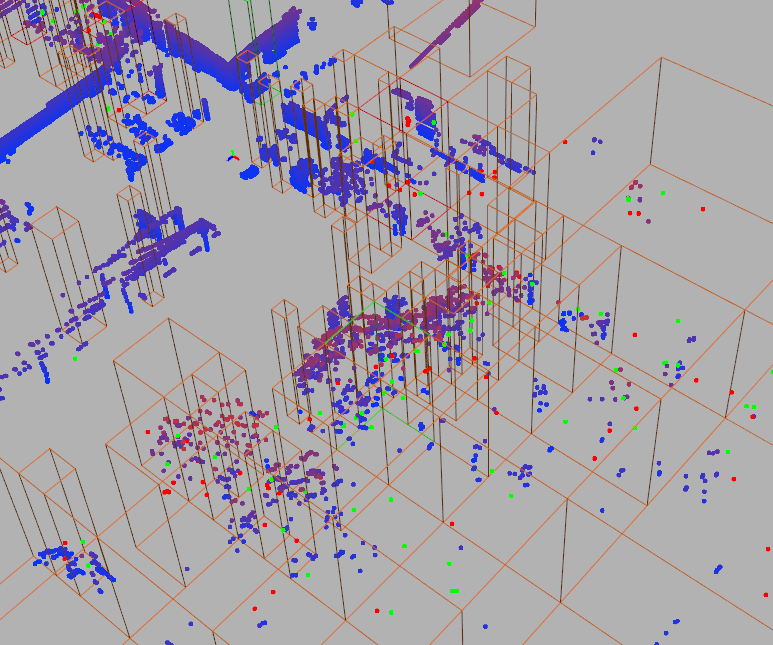
\includegraphics[width=\textwidth]{images/quadTree.png}
			{\small (α) Quadtree (2D)}
		\end{minipage}
		\hfill
		\begin{minipage}{0.48\textwidth}
			\centering
			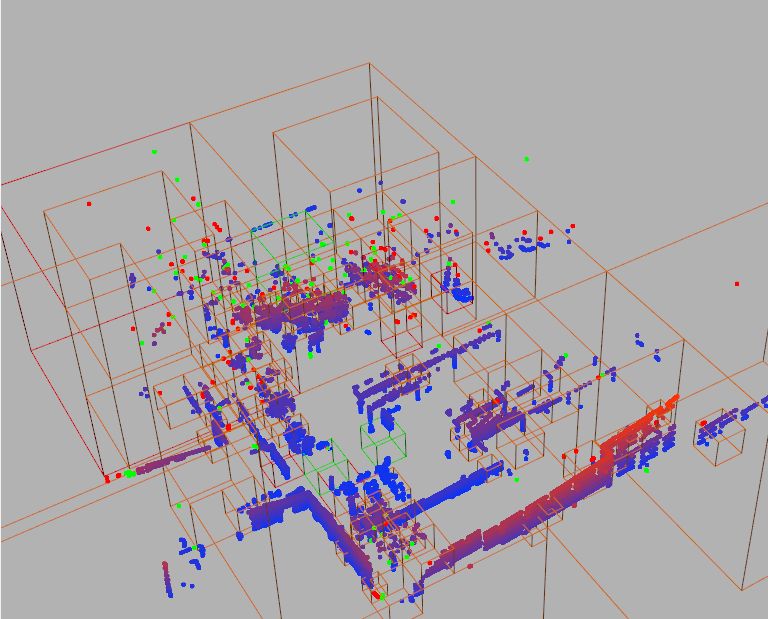
\includegraphics[width=\textwidth]{images/octTree.png}
			{\small (β) Octree (3D)}
		\end{minipage}
		\caption{Ιεραρχική διαμέριση χώρου με Quadtree (2D) και Octree (3D) για τον εντοπισμό περιοχών αλλαγών.}
		\label{fig:subdivision}
	\end{figure}

	\section{ Κατάτμηση και Σημασιολογική Ταξινόμηση Αντικειμένων}
	
	\subsection{Κατάτμηση με Voxel Grid Clustering}
	Η ομαδοποίηση των σημείων σε clusters γίνεται με τον αλγόριθμο DBSCAN. Επειδή η εκτέλεση του αλγορίθμου στα εκατοντάδες χιλιάδες αρχικά σημεία είναι πολύ αργή, εφαρμόζουμε την εξής μέθοδο επιτάχυνσης:
	\begin{itemize}
		\item Υποδειγματοληπτούμε το νέφος σημείων. Έτσι κρατάμε μόνο λίγα σημεία ανά voxel, μειώνοντας δραστικά τον όγκο των δεδομένων.
		\item Εκτελούμε τον DBSCAN πάνω στα downsampled σημεία για να βρούμε τα clusters.
		\item Αντιστοιχίζουμε τα labels των clusters πίσω στα αρχικά σημεία πλήρους ανάλυσης, βρίσκοντας τον πλησιέστερο γείτονα στο downsampled νέφος μέσω ενός KD-Tree.
	\end{itemize}
	Αυτό μας επιτρέπει να έχουμε πολύ γρήγορους χρόνους εκτέλεσης χωρίς να χάνουμε την αρχική ανάλυση των σημείων.
	
	\subsection{Γεωμετρικοί Ευρετικοί Κανόνες και Σημασιολογικές Κατηγορίες}
	Αφού χωρίσουμε τα σημεία σε clusters, κατηγοριοποιούμε το κάθε cluster σε μία σημασιολογική κατηγορία, ελέγχοντας τις διαστάσεις του bounding box του:
	\begin{table}[h!]
		\centering
		\begin{tabular}{|l|c|c|c|}
			\hline
			\textbf{Κατηγορία} & \textbf{Εμβαδόν / Πλάτος} & \textbf{Ύψος} & \textbf{Αναλογία Ύψους / Πλάτους} \\ \hline
			Κτίριο (Building) & $\ge 20\text{ m}^2$ & $\ge 2\text{ m}$ & - \\ \hline
			Άνθρωπος (Human) & $\le 0.8\text{ m}^2$ ($W_x, W_y \le 1\text{ m}$) & $0.8 - 2.1\text{ m}$ & $\ge 1.2$ \\ \hline
			Στύλος (Pole) & $W_x, W_y < 1.5\text{ m}$ & $\ge 1.5\text{ m}$ & $\ge 1.5$ \\ \hline
			Δέντρο (Tree) & $< 25\text{ m}^2$ & $\ge 2\text{ m}$ & - \\ \hline
			Αντικείμενο (Object) & - & - & Default (Άλλο) \\ \hline
		\end{tabular}
		\caption{Γεωμετρικοί ευρετικοί κανόνες για τη σημασιολογική κατηγοριοποίηση των clusters.}
		\label{tab:heuristics}
	\end{table}
	Τα clusters που έχουν πολύ μικρό ύψος απορρίπτονται ως έδαφος που δεν πέρασε το filtering στην αρχή.

	\subsection{Δυναμικά Αντικείμενα}
	
	Για να παρακολουθήσουμε την κίνηση των αντικειμένων στο χρόνο, πρέπει να συσχετίσουμε τα αντικείμενα που εντοπίζονται σε ένα καρέ με αυτά του επόμενου (Object Tracking):
	\begin{itemize}
		\item \textbf{Υπολογισμός Κεντροειδούς:} Για κάθε cluster στο τρέχον καρέ, υπολογίζουμε το κεντροειδές του.
		\item \textbf{Συσχέτιση ανά Κατηγορία:} Συγκρίνουμε το κεντροειδές αυτό μόνο με τα κεντροειδή των αντικειμένων του προηγούμενου καρέ που ανήκουν στην ίδια κατηγορία (π.χ όχημα με όχημα).
		\item \textbf{Κατώφλι Απόστασης:} Αν η Ευκλείδεια απόσταση μεταξύ των κεντροειδών είναι μικρότερη από ένα όριο και είναι η ελάχιστη δυνατή, θεωρούμε ότι πρόκειται για το ίδιο αντικείμενο και του αποδίδουμε το ίδιο ID.
		\item \textbf{Δημιουργία Νέου Track:} Αν δεν βρεθεί κανένα κοντινό αντικείμενο που να πληροί τα παραπάνω κριτήρια, το cluster θεωρείται νέο αντικείμενο και του αποδίδεται ένα καινούριο ID.
	\end{itemize}
	
	\begin{figure}[h!]
		\centering
		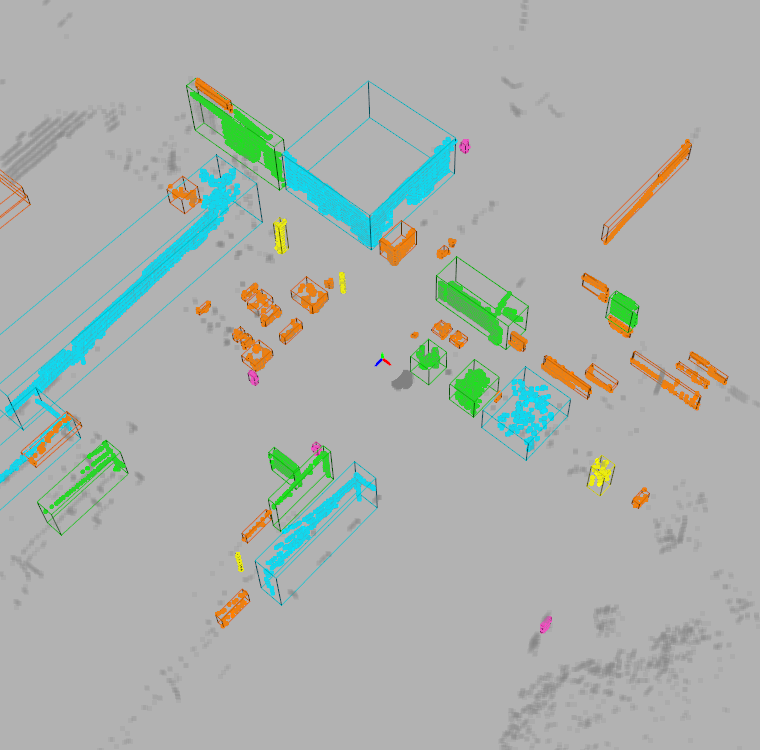
\includegraphics[width=0.8\textwidth]{images/classification.png}
		\caption{Σημασιολογική κατηγοριοποίηση και tracking των αντικειμένων (κτίρια, δέντρα, στύλοι, άνθρωποι, οχήματα) στη σκηνή.}
		\label{fig:classification}
	\end{figure}

	
	\section{Παραμετροποίηση Γεωμετρίας και Πειραματική Μελέτη}
	
	\subsection{Επίδραση Υποδειγματοληψίας}
	Η υποδειγματοληψία είναι απαραίτητη για την ομαλή εκτέλεση της εφαρμογής σε πραγματικό χρόνο:
	\begin{itemize}
		\item Για τα μεγάλα αρχεία LiDAR, η φόρτωση εκατομμυρίων σημείων προκαλεί καθυστερήσεις στο rendering και στην επεξεργασία.
		\item Επιλέγοντας ένα βήμα υποδειγματοληψίας, μειώνουμε τον όγκο των σημείων χωρίς να χάνουμε τη γεωμετρική πληροφορία των βασικών αντικειμένων.
		\item Αν το βήμα είναι πολύ μεγάλο, μικρά αντικείμενα όπως στύλοι ή άνθρωποι χάνουν την πυκνότητά τους και δεν μπορούν να ανιχνευθούν από τον DBSCAN.
	\end{itemize}
	
	\section{Μελλοντικές Επεκτάσεις}
	Για τη μελλοντική βελτίωση και επέκταση της εφαρμογής, προτείνονται τα εξής:
	\begin{itemize}
		\item \textbf{Υποδειγματοληψία Voxel Downsampling:} Αντικατάσταση της απλής υποδειγματοληψίας με βήμα από ένα ομοιόμορφο φίλτρο Voxel Grid κατά την αρχική φόρτωση, ώστε να διατηρείται σταθερή η πυκνότητα των σημείων στο χώρο και να βελτιωθεί η ακρίβεια της ευθυγράμμισης.
	\end{itemize}
	
	\section{Github Repository}
	Ο κώδικας της εργασίας είναι διαθέσιμος στο Github: \\
	\url{https://github.com/jimfil/dynamicScenes}
	\begin{thebibliography}{99}
		\bibitem{learnopencv_icp} LearnOpenCV, "Iterative Closest Point (ICP) Explained," \url{https://learnopencv.com/iterative-closest-point-icp-explained/}.
		\bibitem{scipy_ckdtree} SciPy Documentation, "scipy.spatial.cKDTree," \url{https://docs.scipy.org/doc/scipy/reference/generated/scipy.spatial.cKDTree.html}.
	\end{thebibliography}
	
\end{document}